\documentclass[12pt]{article}
\usepackage{enumerate}
\usepackage{amsmath}
\usepackage{amssymb}
\usepackage{amsthm}
\usepackage{etoolbox}
\usepackage{graphicx}

\newcommand{\Name}[1]{\noindent \textbf{Name:} #1 \\}
\newcommand{\Workedwith}[1]{\noindent \textbf{Worked with:} #1 \\}
\newcommand{\Problem}[3]{\mbox{} \newline \noindent \textbf{\textbf{Problem #1: #2 [#3 Points] \\ }}}


\begin{document}

\begin{center}
  \bf
  Algorithms \\
  CMPT 307 D200 \\
  Spring 2024 \\
  \rm
  Homework 5\\
  Due:  Sunday, Mar 31 at 10:00 PM \\
\end{center}

\Name{Sara Magdalinski}
\Workedwith{N/A}

\Problem{4}{Maxiclip}{20}

Many puzzles can be solved by transforming (or ``reducing'') them to network flow problems.  That's what you'll do here!

Maxiclip, a provider of popular online games, has developed a board game that works like this:  We're given an $n \times n$ board.  Some of the squares are gray and the rest are white.  The goal is to place $n$ tokens on white cells such that every row contains exactly one token and every column contains exactly one token.  Tokens may not be placed on the gray cells.
For example, Figure~\ref{fig:boardgame} shows a board with a valid placement of tokens (indicated by the X marks).

\begin{figure}[h]
\begin{center}
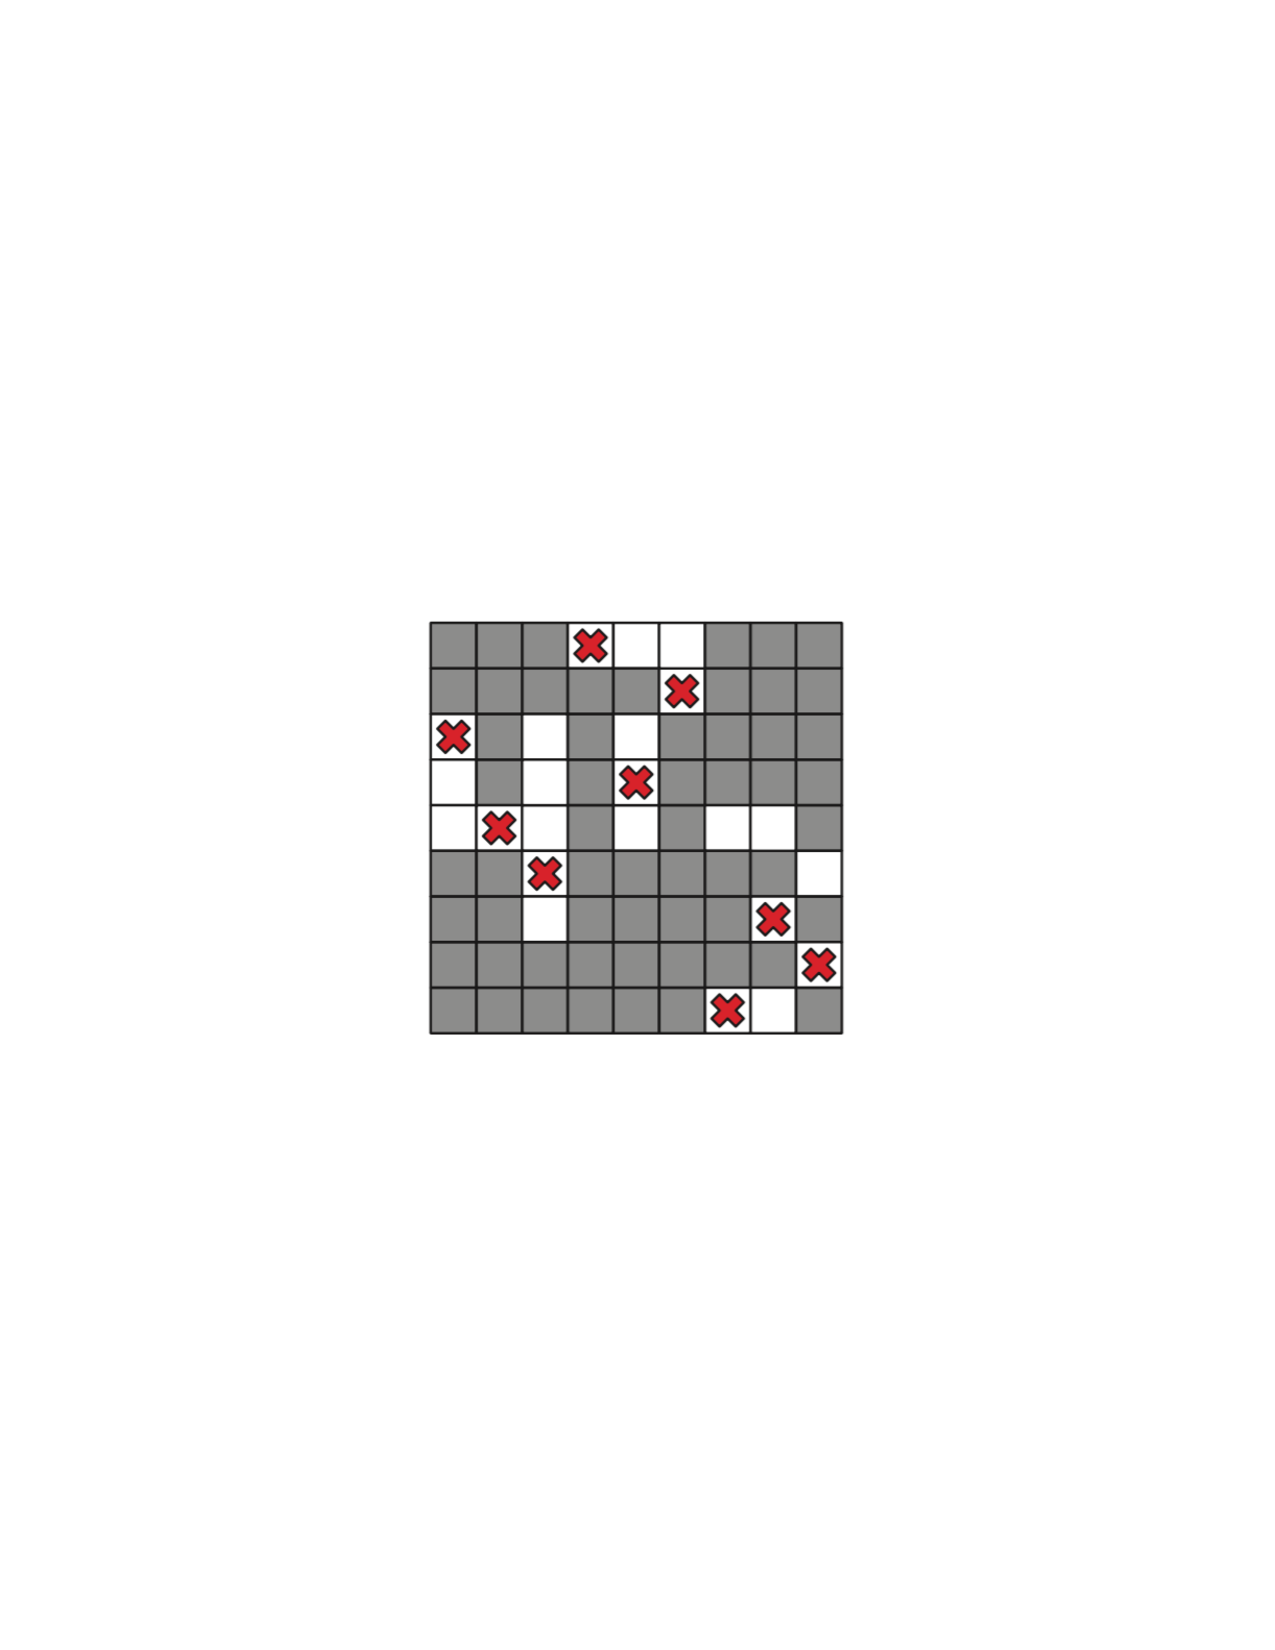
\includegraphics[width=2in]{Board.pdf}
\end{center}
\caption{A square board with a valid placement of tokens.}
\label{fig:boardgame}
\end{figure}

You may assume that the board is represented as follows:  We're given the value of $n$ (the width and heigh to the board) and a list of ordered pairs, each representing the row and column of a white cell in the board.
Using either the Ford-Fulkerson algorithm or the Edmonds-Karp algorithm, describe an efficient algorithm that determines whether or not a given board has a valid solution.  (You don't need to actually give the valid solution if it exists, although you'll see that this is not hard once you can determine whether or not a solution exists.)  Prove that your algorithm is correct and derive its running time as a function of $n$ (and only $n$ -- do not include other terms in the running time).

\textbf{Solution:}\\

Step 1: Reduction:\\

This problem can be represented as a bipartite graph G (V = A $\cup$ B, E) where A and B represent the two distinct vertex sets and can be used to provide a solution using a network flow algorithm. We will let the vertex set A represent the rows and the vertex set B represent the columns. We can label the vertices from 1 through n (dimension of the board) for both sets A and B. We will add edges to represent the white (free) squares on the board. For example, if the square at row 1 column 1 is white we would have an edge from vertex 1 in A to vertex 1 in B (directed). After adding all of these edges, we will then add a vertex, lets call it S to represent the starting node of the network flow and we will add directed edges from S to each vertex in A. We will also add an end node, lets call it N and we will add directed edges from each node in B to N. We will set each edge to have a weight of 1. This problem has now been reduced to a network flow problem and we can solve it using the Ford-Fulkerson algorthm which will determine the maximum flow in the network. We will know a solution is possible if the maximum flow is equal to n since each unit of flow from the source node to the end node represents 1 token being placed at that row and column. If we have a maximum flow of n that means that for each row there is 1 token to be placed and each row will contain a token at a unique column meeting the criteria that each row and and column contain exactly 1 token.\\

Step 2: Proof of Correctness: We can assume by contradiction that the locations of the tokens that we selected is not a valid solution when  we obtained a maximum flow of n. This means that one of the vertexes in A had two outgoing edges and/or one of the vertexes in B had two incoming edges. This is not possible as we only allocated a flow of 1 into each vertex in A and a flow of 1 leaving any vertex in B, therefore it is impossible for any vertex to receive or output a flow greater than 1. Therefore we have a contradiction and we have proved that we have chosen valid positions on the board. To prove that we have selected the maximum number of valid locations on the board we can assume by way of contradiction that there is a larger amount of valid locations than the set of locations where we placed tokens. We could then create a flow through the graph using this higher maximal number of locations, however this is a contradiction since we know that the Ford-Fulkerson algorithm correctly identifies the maximum flow through a graph. Therefore we have also proven that our solution is correct when the algorithm assesses a maximum flow of n.

Step 3: Time Efficiency:  To transform this problem into a network flow problem we need to create nodes for each row and column as well as edges for each cell that is open (white). We know there are n rows and n columns and at most every cell could be white. This gives us a time efficiency of O($n^2 + 2n$) in the worst case for transforming the problem which can be reduced to O($n^2$). \\
We then need to run a maximum flow algorithm. The Ford-Fulkerson algorithm was chosen in this case as it provides the best running time in this situation. It runs in O(E * F) time with e being the number of edges and F being the maximum flow. For this problem we have at most $n^2$ edges representing the white squares plus 2n edges to connect the rows to S and the columns to N. The maximum flow is n based on the way the network flow problem was constructed (since we want to place n tokens on the board). This gives us a running time of O(($n^2 + 2n) * n)$ = O($n^3$).\\

There is no additional running time needed to convert this solution back into the original problem as we must only return that there is a solution if the Ford-Fulkerson algorithm provides a maximum flow of n and that there is no solution in any other case. \\

This gives us an overall running time O($n^2 + n^3$) since these operations are done separately. This can be written as O($n^3$) (the overall running time) when reduced according to Big-O laws.




\end{document}
